\localauthor{Johannes Garstenauer}

\subsection{Schichten}\label{arch:schichten}
Diese Anwendung folgt einer Schichtenarchitektur.
\begin{itemize}
    \item Die \emph{view}-Schicht enthält die Komponenten zur grafischen Darstellung.
    \item Die \emph{control}-Schicht enthält die Komponenten zur Steuerung der grafischen Darstellung und Reaktion auf
    Nutzereingaben.
    \item Die \emph{business}-Schicht enthält die Komponenten, welche die Anwendungslogik umsetzen.
    \item Die \emph{persistence}-Schicht enthält die Komponenten zum Zugriff auf die Datenbasis.
\end{itemize}
Diese Schichten folgen der \emph{\hyperref[arch:mvc]{MVC-Architektur}} wie in \textbf{\hyperref[arch:pakdia]{Abbildung 1}} dargestellt.
Die \hyperref[arch:persistence]{Persistence-} und \hyperref[arch:business]{Businessschichten} gehören hierbei
zum \emph{Model}. Die \hyperref[arch:control]{Controllschicht} stellt den \emph{Controller} dar und die
\emph{Faceletschicht} %todo link
die \emph{View}.

\begin{figure}[H]
\centering
    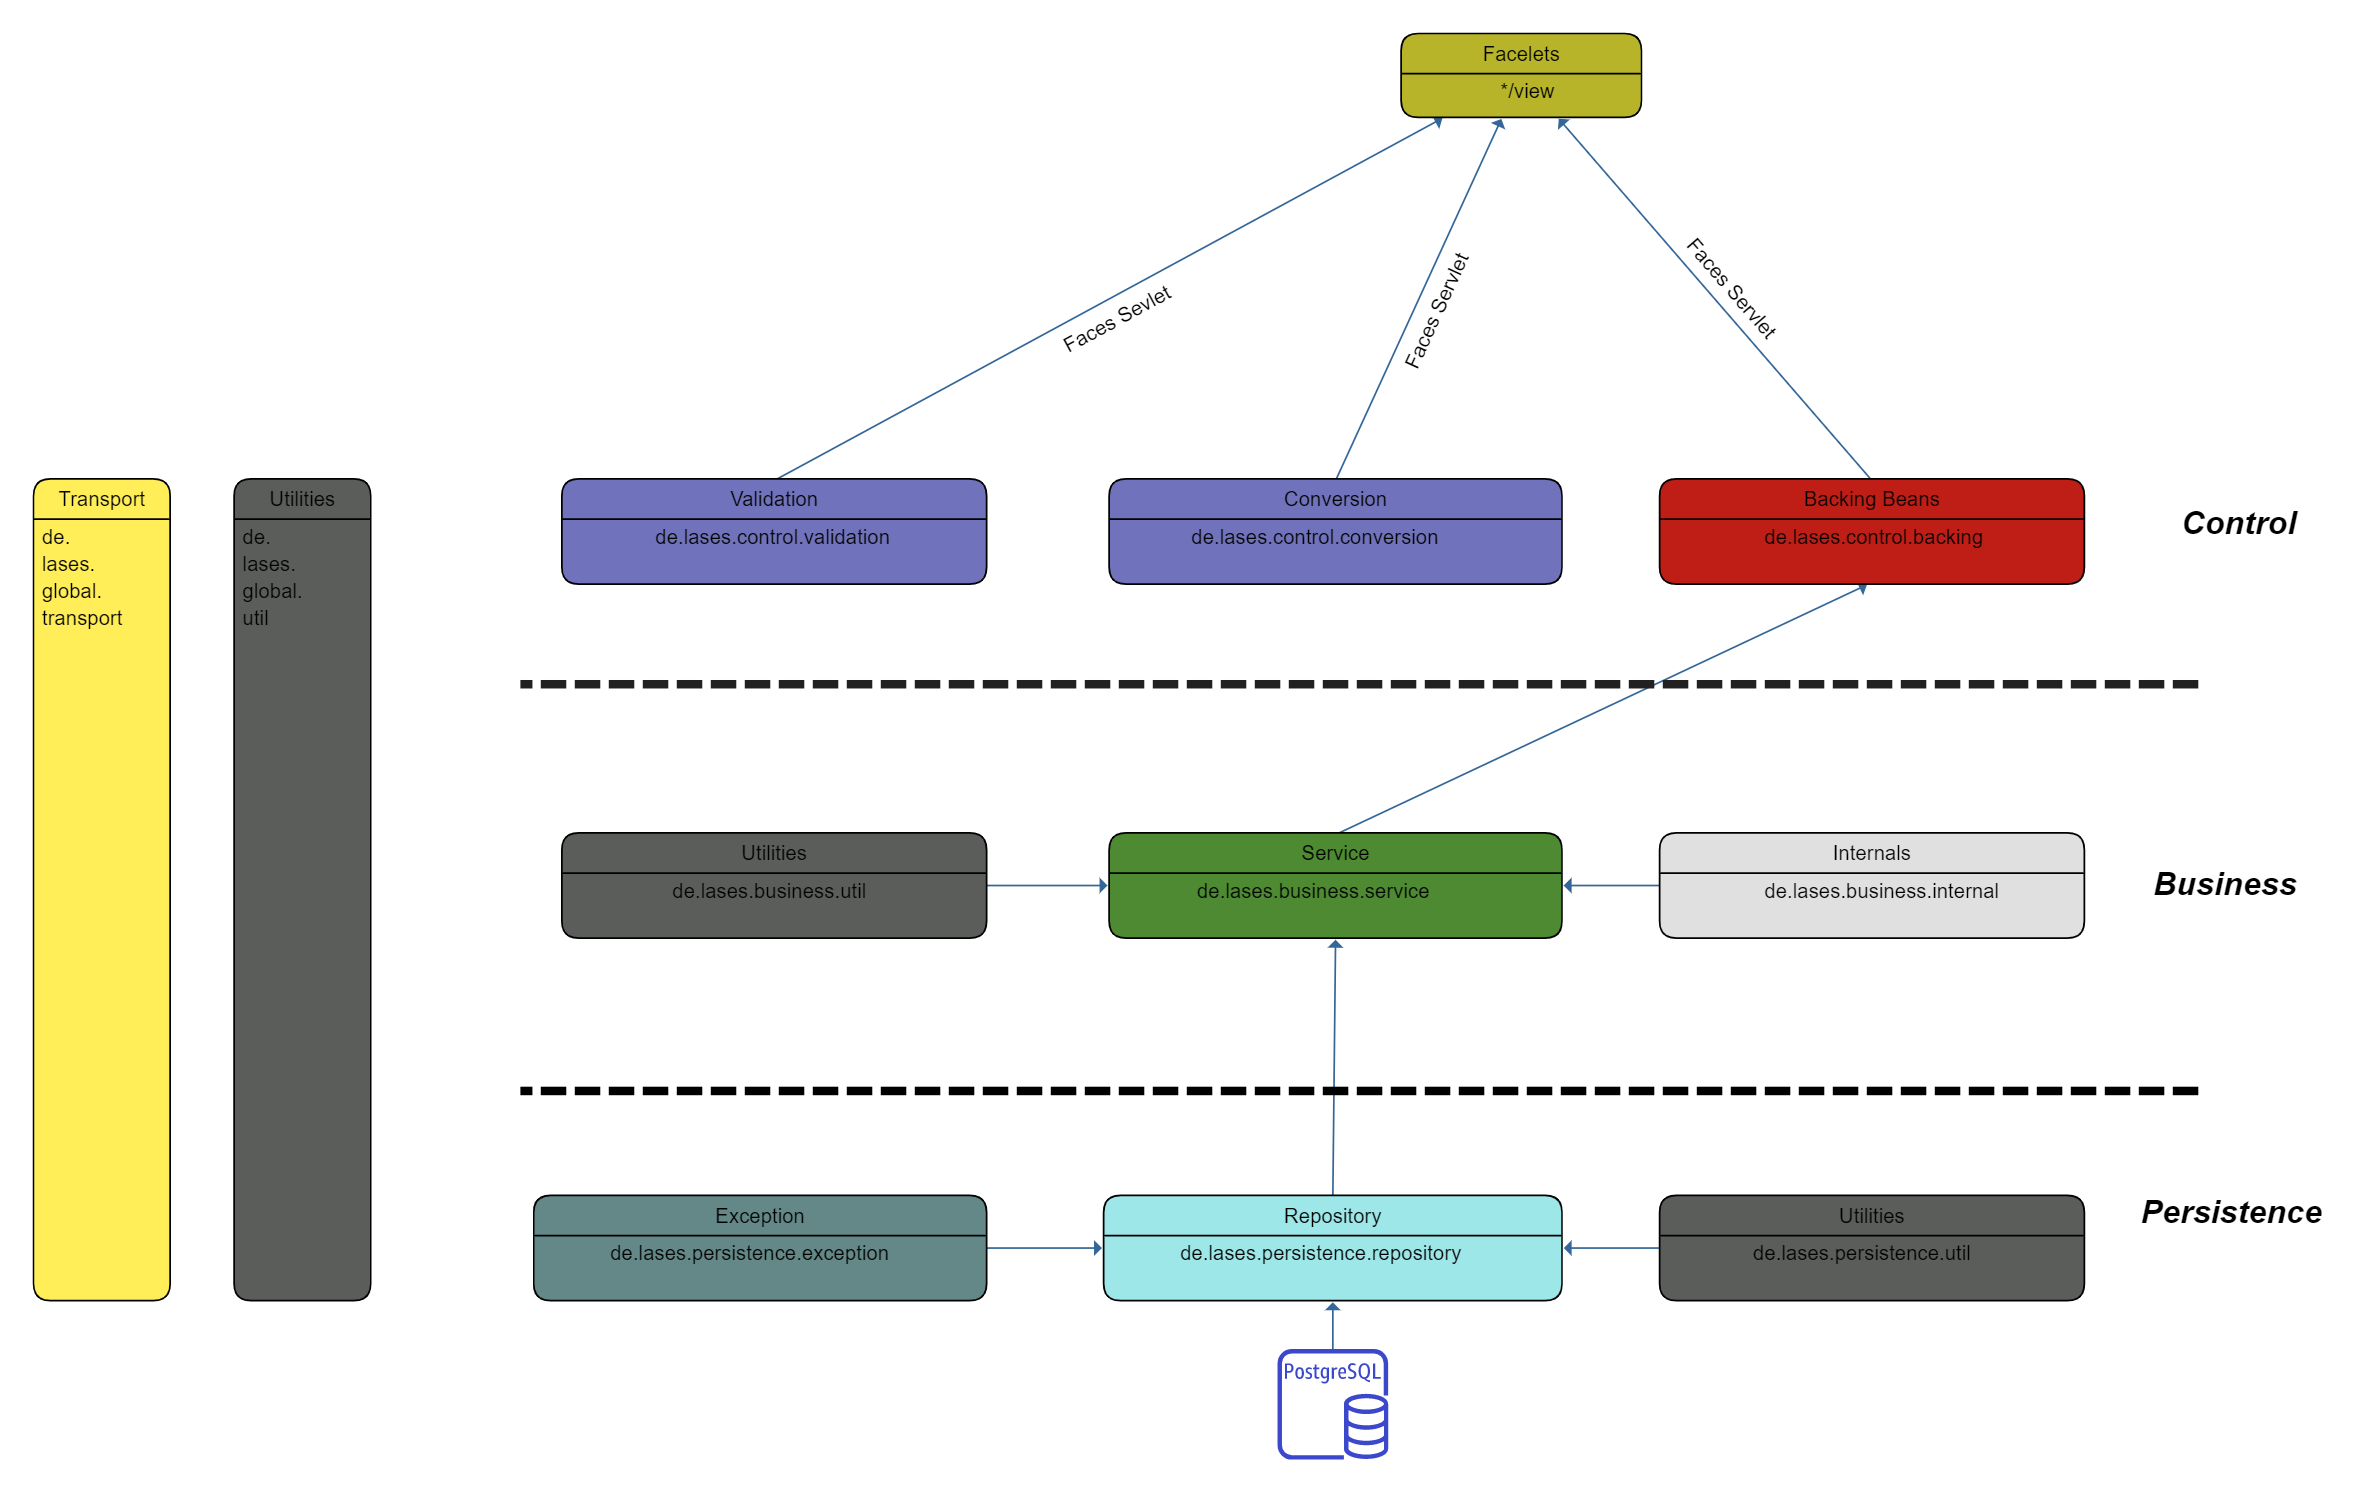
\includegraphics[width=\linewidth]{graphics/Paketdiagramm5.0}\label{arch:pakdia}
    \caption{Das Schichtenmodell der LasEs-Anwendung.}
\end{figure}

%todo mvc sichtbar machen.
%todo view einfügen
%todo servlets?

\subsection{Pakete}\label{arch:pakete}

\subsubsection{de.lases.control} \label{arch:control}
Dieses Paket enthält alle Klassen der Kontrollschicht.
\newline\newline
\textbf{\emph{de.lases.control.conversion}}
enthält alle Klassen, die zur Konvertierung von Nutzereingaben
in Facelets verwendet werden.
\newline\newline
\textbf{\emph{de.lases.control.validiation}}
enthält alle Klassen, die zur Validierung von Nutzereingaben
in Facelets verwendet werden.
\newline\newline
\textbf{\emph{de.lases.control.backing}}\label{arch:backing}
enthält alle Managed Beans welche zur Darstellung der Facelets aus der
%todo link
View Verwendung finden. Zu jedem Facelet [facelet] existiert genau ein
Backing-Bean, welches [facelet]Backing genannt wird.
%todo
%\subsubsection*{edu.uni_passau.lases.control.servlet}

\subsubsection{de.lases.business}\label{arch:business}
Dieses Paket enthält alle Klassen der Anwendungslogikschicht.
\newline\newline
\textbf{\emph{de.lases.business.service}}\label{arch:service}
enthält alle Klassen, die den Hauptteil der Anwendungslogik umsetzen.
Das sind also alle Dienste welche den
\hyperref[arch:backing]{Backing Beans} zur Verfügung
gestellt werden und auf die auf die %todo link repos
Repositories zugreifen.
\newline\newline
\textbf{\emph{de.lases.business.util}}
enthält die Hilfsklassen, welche Dienste zur Verfügung stellen,
die von der Anwendungslogik selbst getrennt werden können.
\newline\newline
\textbf{\emph{de.lases.business.exception}} \label{arch:busex}
enthält die Exceptionklassen, die ein Fehlverhalten im System repräsentieren.
\newline\newline
\textbf{\emph{de.lases.business.internal}}
enthält die Klassen, welche zur internen Verwaltung verwendet werden.
Hierzugehört beispielsweise die Sessionverwaltung, sowie der Systemstart und -stop.

\subsubsection{de.lases.persistence}\label{arch:persistence}
Dieses Paket enthält alle Schichten der Persistenzschicht.
\newline\newline
\textbf{\emph{de.lases.persistence.repository}}\label{arch:repository}
enthält alle Klassen, die dem direkten Zugriff auf die Datenbank dienen.
\newline\newline
\textbf{\emph{de.lases.persistence.util}}
enthält die Hilfsklassen zur Datenbankverwaltung, wie einen
Connection-Pool.
\newline\newline
\textbf{\emph{de.lases.persistence.exception}}
enthält die Exceptionklassen, welche ein Fehlverhalten im Umgang mit der
Datenbasis repräsentieren.

\subsubsection{de.lases.global}
Dieses Paket enthält alle Klassen welche über mehrere Schichten hinweg
verwendet werden.
\newline\newline
\textbf{\emph{de.lases.global.logging}}
enthält Hilfsklassen für schichtenübergreifende Loggingfunktionen.
\newline\newline
\textbf{\emph{de.lases.global.transport}}\label{arch:transport}
enthält alle POJO-Klassen, die Daten in der Anwendung repräsentieren und zu deren
Transport verwendet werden.

%todo i18n resource bundles: info (tooltips), names (labels), messages (facesmsg)

\subsection{Fehlerbehandlung}
Bei Verwendung der Anwendung können Fehler auftreten. Diese werden zur Nachvollziehbarkeit
immer geloggt. Daraufhin wird auf verschiedene Weisen verfahren.

\subsubsection{Geprüfte Ausnahmen}
Geprüfte Ausnahmen repräsentieren Ausnahmesituationen, mit
denen gerechnet werden muss und auf die reagiert wird.
Treten solche auf, dann werden sie mit einer
\hyperref[arch:busex]{Ausnahmeklasse} und Fehlermeldung
an den Aufrufer weiterpropagiert.
In \hyperref[arch:service]{Service-Klassen} werden auftretende Ausnahmen weiter zu den
\hyperref[arch:backing]{Backing-Beans} propagiert, wo FacesMessages %todo link
generiert werden.
Diese werden dann von den zugehörigen Facelets %todo link
gerendert.

\subsubsection{Ungeprüfte Ausnahmen}
Bei ungeprüften Ausnahmen handelt es sich um fatale Fehler, wie sie beispielsweise durch
Programmierfehler entstehen können. Diesen werden vom anwendungsweiten
ExceptionHandler %todo link
aufgegriffen. Der User wird daraufhin auf die Fehlerseite %todo link
weitergeleitet.
%todo stacktrace wirklich drinnen lassen oder offensichtliche Kopie?

\subsection{Frameworks}\label{arch:frameworks}

\subsubsection{Jakarta Server Faces}
Jakarta Server Faces (JSF; früher JavaServer Faces) ist ein Framework-Standard zur
Entwicklung von grafischen Benutzeroberflächen für Webanwendungen in Java, basierend auf Servlets und JSP-Technik.
Es wird die Referenzimplementierung \emph{Mojarra} verwendet.

\subsubsection{Context and Dependency Injection}
Die \emph{Context and Dependency Injection} ist eine Technologie welche die
Abhängigkeitsverwaltung zwischen Objekten vereinfacht. Im Sinne der
\emph{Inversion of Control} werden dem Entwickler Werkzeuge an die Hand gelegt, mithilfe derer
er Objektrefernzierung tätigen kann, ohne diese Objekte vorher explizit zu erstellen.
Diese referenzierten Objekte können in andere Objekte zur Laufzeit \emph{injiziert} werden.
Somit können Objekte in dieser Anwendung ohne Initialisierung oder umständlichen Transport der Referenzierung
verwendet werden.
Dies ermöglicht eine losere Kupplung zwischen Klassen und somit Erweiterbarkeit
und Austauschbarkeit.
Die \emph{CDI} verwaltet in dieser Anwendung alle Objekte der \hyperref[arch:backing]{Backing-Beans}
und \hyperref[arch:service]{Services}.
Es wird die Referenzimplementierung \emph{Weld} von \emph{JBoss} verwendet.

\subsection{Patterns}\label{arch:patterns}
%todo konkret auf unser System abstimmen. (Keine allg. erklärung der patterns)

\subsubsection{Model View Controller}\label{arch:mvc}
Dieses Entwurfsmuster trennt die Klassen und Komponenten der Anwendung in drei
verschieden Teile, welche jeweils eigene Aufgaben übernehmen:
\begin{itemize}
    \item Die \emph{\textbf{View-Komponenten}} übernehmen alle Aufgaben,
    welche mit der grafischen Darstellung der Anwendung zusammenhängen.
    In dieser Anwendung sind dies die Facelets. %todo link facelets
    \item Die \emph{\textbf{Controller-Komponenten}} übernehmen alle Aufgaben,
    welche die Interaktion zwischen der View und dem Model betrifft. Sie behandeln
    Nutzereingaben, Validation und Konvertierung etc. In dieser Anwendung befinden sie
    sich in den \hyperref[arch:control]{edu.uni\_passau.lases.control} Paketen.
    \item Die \emph{\textbf{Model-Komponenten}} beinhalten die Modelldaten, sowie jene
    Klassen welche sich mit deren Beschaffung und Verarbeitung beschäftigen. In dieser
    Anwendung befinden sie sich in den \hyperref[arch:business]{edu.uni\_passau.lases.business}
    und \hyperref[arch:persistence]{edu.uni\_passau.lases.persistence} Paketen.
\end{itemize}
Die Verwendung dieses Patterns bietet viele Vorteile hinsichtlich der Modularität
und Erweiterbarkeit der Anwendung.

\subsubsection{Singleton}
Eine Klasse, welche nach dem Singleton-Entwurfsmuster implementiert wurde zeichnet
sich dadurch aus, dass es nur genau eine Instanziierung von dieser Klasse geben
kann und darf. Hierdurch werden vorrangig Ressourcen gespart, außerdem wird die
Verwaltung der im Objekt gekapselten Funktionalität erleichtert.
Ein Beispiel hierfür ist der Connection Pool, damit sichergestellt wird, dass
eine genau festgelegte Anzahl an Datenbankverbindungen existiert und nicht mehr.

\subsubsection{Data Transfer Object}
Dieses Entwurfsmuster schreibt die Verwendung von \emph{Data Transfer Objects}
zur einheitlichen Darstellung der Entitäten in den Modelldaten und dem Transport
von Daten vor.
Diese sind POJOs, welche private Felder zur Repräsentation der Daten mit Getter- und
Settermethoden haben.
Der Vorteil der Verwendung dieses Entwurfsmusters liegt darin, dass eine
einheitliche und übersichtliche Schnittstelle für Datenrepräsentation und Transport
in der Anwendung besteht. Die zugehörigen Klassen lagern im
\hyperref[arch:transport]{edu.uni\_passau.lases.transport} Paket.

\subsubsection{Repository}
Beim \emph{Repository} Pattern wird für jedes Business-Objekt oder jede Entität
eine Klasse definiert welche den Datenbankzugriff auf die zugehörigen Daten steuert.
Für diesen Zugriff werden oft die \textit{CRUD}-Methoden, das heißt
\begin{itemize}
    \item \textit{CREATE} zur Erstellung,
    \item \textit{READ} zum Erhalten,
    \item \textit{UPDATE} zum Updaten,
    \item und \textit{DELETE} zum Löschen
\end{itemize}
eines oder mehrerer Datenbankeinträge der zugehörigen Entität, angeboten.
Weiterhin findet das Mapping auf die \hyperref[arch:transport]{DTO-Objekte} dieser Anwendung statt.
In dieser Anwendung finden sich die \emph{Repository-Pattern} Klassen im Paket
\hyperref[arch:repository]{edu.uni\_passau.lases.repository}. Durch die mit
der Verwendung dieses Patterns gewonnenen Übersichtlichkeit erleichtern wir uns die
Implementation und ermöglichen leichte Erweiterbarkeit der Datenschemas.

\subsubsection{Object Pool}
Das \emph{Object Pool} Erzeugungsmuster wird dazu verwendet, Objekte nach initialer Erzeugung
vorzubehalten, da dies sinnvoller ist als sie bei jeder Verwendung neu zu erzeugen.
Somit werden Ressourcen gespart. In dieser Anwendung findet dieses Entwurfsmuster
beim Connection Pool %todo link
Verwendung und bietet den zusätzlichen Vorteil, dass eine feste Maximalanzahl an
Datenbankverbindungen festgelegt werden kann.

\subsubsection{Observer}
Das \emph{Observer} Verhaltensmuster beschreibt Methoden, welche auf
Änderungen im Zustand eines Systems warten und daraufhin handeln.
In unserem System findet das beispielsweise beim LifeTimeListener %todo link
zur Reaktion auf das Herunterfahren oder Starten des Systems Verwendung.
%todo propagation der messages aus service in backingbeans